\documentclass[10pt,aspectratio=169, compressed]{beamer}
\usetheme{boxes}
\usecolortheme{default}
\usepackage{kotex}
\definecolor{qualityblue}{RGB}{222,232,242}
\definecolor{qualityred}{RGB}{243,224,224}
\definecolor{qualityblue}{RGB}{135,215,128}
\definecolor{qualityred}{RGB}{243,137,106}
\definecolor{celldarkgray}{RGB}{80,80,80}

% Custom colors
\definecolor{darknavy}{RGB}{30,39,97}
\definecolor{iceblue}{RGB}{202,220,252}
\definecolor{accentred}{RGB}{180,50,50}
\definecolor{darkgray}{RGB}{60,60,60}
\definecolor{lightgray}{RGB}{240,240,240}
\definecolor{forestgreen}{RGB}{34,120,60}

\setbeamertemplate{itemize item}[ball]
\setbeamertemplate{itemize subitem}[ball]
\setbeamertemplate{itemize subsubitem}[ball]
\setbeamertemplate{enumerate item}[ball]
\setbeamertemplate{enumerate subitem}[ball]
\setbeamertemplate{enumerate subsubitem}[ball]

\setbeamercolor{block title alerted}{fg=white,bg=accentred}
\setbeamercolor{block body alerted}{bg=accentred!8}
\setbeamercolor{block title example}{fg=white,bg=forestgreen}
\setbeamercolor{block body example}{bg=forestgreen!8}
\setbeamercolor{itemize item}{fg=darknavy}
\setbeamercolor{itemize subitem}{fg=darknavy!70}
\setbeamercolor{block title}{fg=black,bg=gray!15}
\setbeamercolor{block body}{fg=black,bg=gray!5}

\setbeamertemplate{navigation symbols}{}
\setbeamertemplate{footline}{%
  \hfill\insertframenumber/\inserttotalframenumber\hspace{4mm}\vspace{2mm}%
}

\usepackage{amsmath,amssymb,amsthm}
\newcommand{\mathbbm}[1]{\mathbf{#1}}
\usepackage{mathtools}
\usepackage{tikz}
\usetikzlibrary{arrows.meta,positioning,calc,decorations.pathreplacing,shapes}
\usetikzlibrary{tikzmark}
\usepackage{booktabs}
\usepackage{hyperref}
\usepackage{appendixnumberbeamer}
\usepackage{subcaption}
\usepackage{graphicx}


\usepackage{cancel}


\DeclareMathOperator*{\argmax}{argmax}
\DeclareMathOperator*{\argmin}{argmin}

\newtheorem{proposition}{Proposition}

\newcommand{\backupbegin}{
   \newcounter{framenumberappendix}
   \setcounter{framenumberappendix}{\value{framenumber}}
}
\newcommand{\backupend}{
   \addtocounter{framenumberappendix}{-\value{framenumber}}
   \addtocounter{framenumber}{\value{framenumberappendix}} 
}

\title{\ \\[0.2em]
\LARGE Pay to Quit\\[0.5em]
\large Robust Team Incentives with Hidden Need\\[0.3em]
}
\author{%
\begin{tabular}{c@{\hspace{1.5cm}}c}
Hyungmin Park & Youngji Sohn \\[0.5em]
{\small University of Oslo} & {\small University of Warwick}\\[-0.5em]
\end{tabular}
}
%\author[Park \& Sohn]{Hyungmin Park \quad\quad\quad Youngji Sohn\\[-0.5em]}
%\institute[]{\small  University of Oslo \quad\quad\quad University of Warwick\\[0.5em] }
\date{\small [35min] \quad %EETC \quad 
September 2026}


\usepackage{colortbl,hhline}
\begin{document}

\frame[noframenumbering]{\titlepage}


%=============================================================
% MOTIVATION
%=============================================================

\begin{frame}{Team project with hidden need}

A project consists of interdependent parts that differ in their \textcolor{blue}{\emph{initial quality}}.

\bigskip

Each expert privately inspects the initial quality of the part:
\begin{itemize}
    \item Some parts are already \textcolor{blue}{\emph{satisfactory}}: no need to repair.
    \item Some parts are \textcolor{blue}{\emph{faulty}} and require repair.
\end{itemize}

\medskip

Each expert privately chooses whether
\begin{itemize}
	\item to make a \emph{costly effort} to repair
	\item or to \emph{leave} it as it is.
\end{itemize}

\bigskip

\mbox{For example: a software update release, a medical team, a consulting team, and remedial repairs.}

\end{frame}





\begin{frame}{What does the manager do?}
% 일반적으로 이렇다
% 왜냐면 참가하는건 최소한 일을 하는게 옵션인데
% 옵트아웃하는건 일을 안한다는 이야기고, paying them feels wasteful.

{A natural contract}: \ pay only experts who \emph{\textcolor{blue}{undertake}} the repair task.

\smallskip

\begin{itemize}
  \item Experts with satisfactory parts also want the bonus.
  \item Undertaking the task does not distinguish productive repair from unnecessary presence.
%  \item In team production, uncertainty about others' quality makes effort more costly to induce.
  \end{itemize}


\bigskip

What is an optimal way to induce high-quality parts in such a team project?\\


\end{frame}






\begin{frame}{This paper}

{Setting.}\quad Team production with complementarities, hidden need, and unobservable effort

\medskip

{Objective.}\quad
Robustly induce high quality in every part at the minimum cost.
%robust 살짝 이야기 설명 하고 그 담에 왜 belief-free approach를 쓰는지 살짝 설명
%Ensuring all parts achieve high quality, robustly to players' beliefs about other parts
%\phantom{\textbf{Objective.}\quad} about others'  and actions

\medskip

{Solution concept.}\quad Belief-free rationalizability (Bergemann \& Morris, 2017)

\medskip

{Finding.}\quad The optimal contract is pay-to-quit.

\medskip

\medskip

\medskip

\medskip

{Today.}\quad Focus on fault-repair technology

\end{frame}






\iffalse



\begin{frame}{Preview: When only 3/5 needs fixing}
\ \\ \ 
\begin{figure}[h!]
\begin{subfigure}[b]{.49\linewidth}
\centering
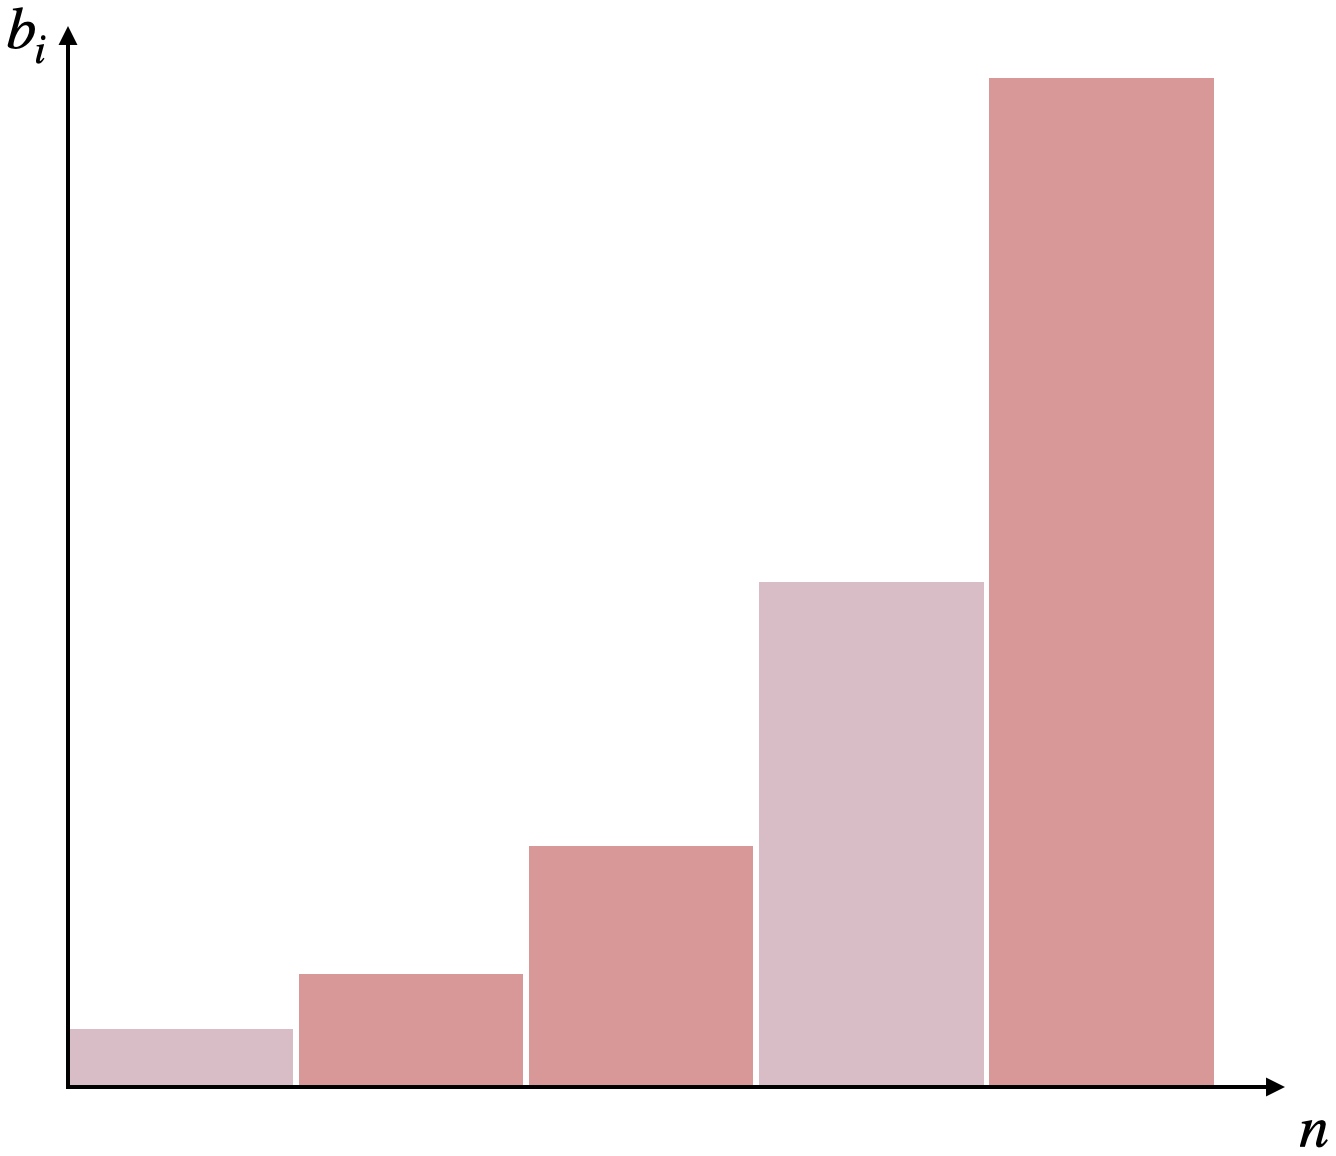
\includegraphics[width=\linewidth]{1PO}

\end{subfigure}\hfill
\begin{subfigure}[b]{.49\linewidth}
\centering
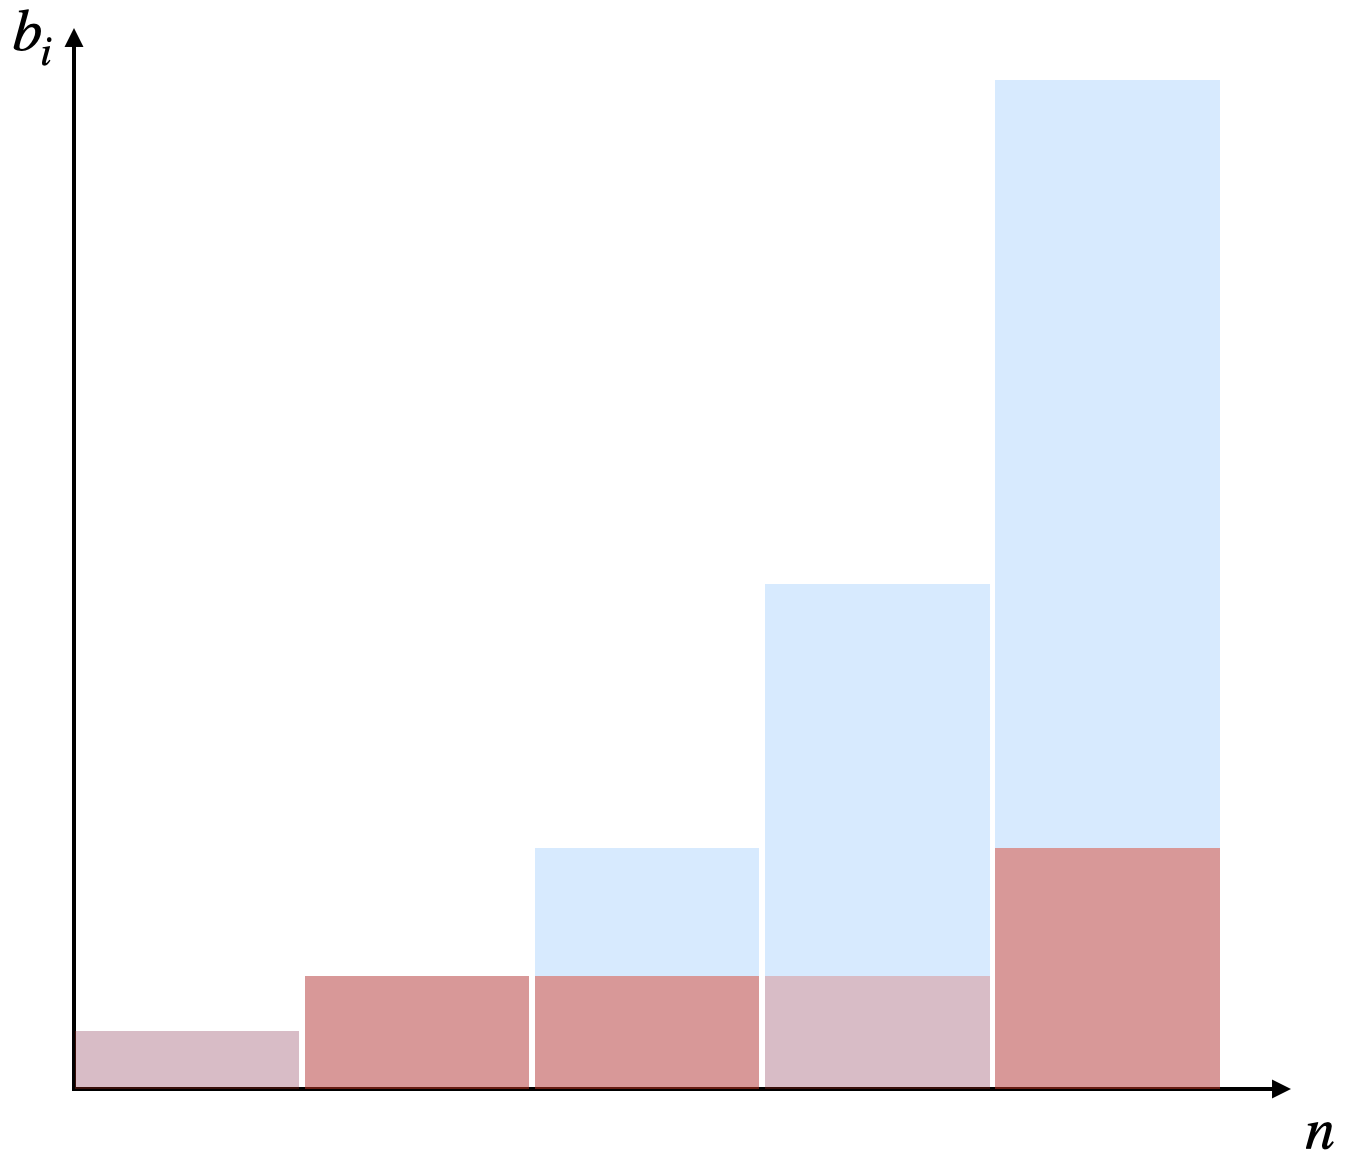
\includegraphics[width=\linewidth]{1PtQ}

\end{subfigure}%
%\caption{name A and B \subref{AAA}\subref{BBB}}
\end{figure}

\end{frame}

\fi



%=============================================================
% EXAMPLE
%=============================================================



\begin{frame}[plain, noframenumbering]
\centering
\vfill
{\large Model with symmetric $n=2$}
\vfill
\end{frame}




\begin{frame}{Team project}
A project is managed by two experts, $i \in  \{1,2\}$.
\medskip

Each Expert $i$:

%구체적으로 적으라 task type? task initial type?
\begin{itemize}
\item {Task type:}  initial part quality $\theta_i$ is faulty $L$ or satisfactory $H$, with $\Pr(\theta_i = H) = p\in (0,1)$.
\item {Effort:} chooses $e_i \in \{W,S\}$, where $W$ denotes repair at cost $c$ and $S$ denotes no effort.
\end{itemize}

\medskip

{Part quality}
$$q_i = q(\theta_i, e_i) = \begin{cases} q_H & \text{if } \theta_i = H \\
q_H & \text{if } \theta_i = L \text{ and } e_i = W \\
q_L & \text{if } \theta_i = L \text{ and } e_i = S
\end{cases}$$
\hfill ...Fault-repair technology
\smallskip

{Project success}
$$P(\{1,2\}) = 1, \qquad P(\{1\}) = P(\{2\}) = \tfrac{1}{2}, \qquad P(\varnothing) = \tfrac{1}{4}$$
\textcolor{gray}{\small Individual part qualities are complementary.}
\end{frame}






%%%HERE how to explain simultaneous and observation more naturally and make the slide simple?

\begin{frame}{Team project}
%Abstract title -> context lost -> 지들 멋대로 생각합니다. 구체적으로 하십시오. 말랑말랑한 말로 하십시오
%게임이론 교과서는 쓰지 마십시오

\begin{enumerate}
\item Each expert privately observes the task type $\theta_i$.
\smallskip

\item Then, chooses whether to undertake the task ($a_i = 1$) or opt out ($a_i = 0$).

\begin{itemize}
  \item $a_i = 1$: Experts undertaking the task privately choose effort $e_i \in \{W, S\}$.\\[0.2em]
  \item $a_i = 0$: Opting out is effectively $e_i = S$.
\end{itemize}
$\to$ Actions: $(a_i, e_i) \in \{(0,S),\, (1,W),\, (1,S)\}$

\smallskip

\item The project succeeds with $P(Q)$, where $Q$ is the exact set of parts with $q_H$.\\
	Everyone observes the project outcome and task undertaking profile $\mathbf a = (a_1, a_2)$.
\end{enumerate}
\medskip



\textcolor{gray}{\small
We analyze a simultaneous-move game, 
where the undertaking profile $\mathbf a = (a_1, a_2)$ is observed ex post.}

\smallskip

\bigskip

\mbox{{Key feature}: opting out reveals no effort $\Rightarrow$ Undertaking choice \textcolor{blue}{partially verifies} effort choice.}

\bigskip
\smallskip


%스푼 피딩 + 구렁이 담 넘어가는
\end{frame}





\begin{frame}{Principal's problem}
\mbox{The manager aims to achieve \textcolor{blue}{all-high-quality} ($q_1 = q_2 = q_H$)
in  {every outcome} {at} {minimum cost}.}

\bigskip


{Contract:}\quad Bonus $b_i(\mathbf{a}) \geq 0$, conditioned on {the undertaking profile} and {the project outcome}


\bigskip

{Payoff and cost:}\quad Let $Q = \{j : q_j = q_H\}$.
\medskip

\quad\quad {Expert $i$'s payoff} given a realization $(\boldsymbol{\theta}, \mathbf{a}, \mathbf{e})$:
$$u_i = P(Q)\,b_i(\mathbf a) \;-\; c\,\mathbbm 1\{e_i = W\}$$ 
\medskip

\quad\quad {Principal's expected cost} under $\mathbf{p}$:
$$
C_{\mathbf p}(\mathbf{b}) = \mathbb{E}_{\mathbf{p}}\left[P(Q) \cdot \sum_{i \in N} b_i(\mathbf{a})\right]
$$


\end{frame}






\iffalse


\begin{frame}[label=solutionconcept]{Solution concept?}

\textbf{Challenge:} Complementarities $\implies$ multiple equilibria\\
\quad \quad \quad \quad \quad \ \!Uncertainty about others' \textbf{types} and \textbf{actions} interacts

\bigskip

\textbf{Belief-Free Rationalizability} (Bergemann \& Morris, 2017):
\hfill\hyperlink{BFRdef}{\beamergotobutton{Def.}}
\\[0.5em]
For each expert and for each type, iteratively eliminate actions that are never a best response\\
for  \textcolor{red}{\textbf{any arbitrary belief}} over others' surviving types and actions.

\medskip

\begin{itemize}
  \item ``Belief-free'': beliefs over others' types and actions are unrestricted\\
  \phantom{``Belief-free'': }no prior, no consistency with a type space
  \item Very \textcolor{blue}{permissive} solution concept
\end{itemize}



\bigskip

\textbf{Unique implementation under BFR:}\\[0.6em]
All-high-quality outcome uniquely survives, regardless of what Experts believe about each other. \\[0.5em]
 \textcolor{red}{{very robust}}

\end{frame}
\fi




\iffalse
How to separate robustly?
  
  누군가 need가 있어서 일을 하는지,
  누군가 need가 있는데 일을 안하는지
  누군가 need가 없는지
  구분이 불가능합니다.
   니드가 있는 애들은 일을할라면, quality comp  요 세가지에 대해서 다른 놈들이 어떤 상황에 해당되는지에 대한 빌리프에 따라 적절한 행동을 할수도 안하려고 할수도 있어요. 그래서 eq multiplicity가 다른 팀원의 타입과 행동에 대한 빌리프에 따라 생깁니다.
  그런데 In organization, information is dispersed and Experts may hold different beliefs 이런 문제가 있어요.
  common prior assumption은 implementation이 빠게지기 쉬워요.
  니가 오너이고 엄청 비싼 뭐시기를 고치고 있는데, 어떻게 확실하게 implement를 하겠어요?
  그래서 우리는 belief free approach 합니다.

아래의 내용을 이걸로 바꿔버려라.
\fi


\begin{frame}{Remark. Team project}
In a team project: 
\smallskip

\begin{enumerate}
\item An expert with a faulty part faces uncertainty about the other part's quality:
\begin{itemize}
    \item $q_H$: already satisfactory or faulty but repaired.
    \item $q_L$: 	faulty and unrepaired.
\end{itemize}

\medskip

\item Because parts' qualities are complementary, the same contract may support:
\begin{itemize}
    \item Repair under optimistic beliefs about the other parts.
    \item No repair under pessimistic beliefs.
\end{itemize}

\medskip

\item In an organization, information is dispersed across experts, and their beliefs about other parts may differ.
\end{enumerate}
\end{frame}







\begin{frame}[label=solutionconcept]{Robust implementation}

\textbf{Objective:} every part reaches high quality in every rationalizable outcome.

\medskip

%The contract must induce repair of faulty parts without assuming that Experts share a common prior.
%Any intended separation through undertaking must also be robust to their beliefs.

\bigskip

\textbf{Belief-Free Rationalizability} (Bergemann \& Morris, 2017)
\hfill\hyperlink{BFRdef}{\beamergotobutton{Def.}}


For each expert of each type, iteratively eliminate actions that are never best replies \\
    to any arbitrary belief over others' surviving types and actions.
%    \item Require every surviving action profile to yield high quality in both parts.


\medskip

{\small This also rules out BNE with low-quality parts under any common prior.}

\end{frame}



\begin{frame}{\ }
\begin{center}
\setlength{\tabcolsep}{8pt}
\renewcommand{\arraystretch}{1.2}
\scalebox{0.85}{%
\begin{tabular}{r|c|c|c|}
    \multicolumn{1}{r}{$(a_i,e_i)$\quad\ }
    & \multicolumn{1}{c}{\makebox[2.5cm]{Opt out}}
    & \multicolumn{1}{c}{\makebox[2.5cm]{Undertake \& Shirk}}
    & \multicolumn{1}{c}{\makebox[2.5cm]{Undertake \& Work}} \\
    \multicolumn{1}{l}{\quad\quad \ \ $\theta_i$}
    & \multicolumn{1}{c}{$(0,S)$}
    & \multicolumn{1}{c}{$(1,S)$}
    & \multicolumn{1}{c}{$(1,W)$} \\[3pt]
    \hhline{~|-|-|-|}
    Initial high quality $H$ & \cellcolor{qualityblue}$q_H$\rule[-0.45cm]{0pt}{1.1cm} & \cellcolor{qualityblue}$q_H$ & \cellcolor{qualityblue}$q_H$ \\
    \hhline{~|-|-|-|}
    Initial low quality $L$ & \cellcolor{qualityred}$q_L$\rule[-0.45cm]{0pt}{1.1cm} & \cellcolor{qualityred}$q_L$ & \cellcolor{qualityblue}$q_H$ \\
    \hhline{~|-|-|-|}
\end{tabular}
}
\end{center}
\end{frame}



\iffalse
\begin{frame}[label=solutionconcept]{Informational limit}

The manager aims to make all Experts who need to repair to make effort to repair as a unique outcome.

But workers' incentive depends on their beliefs about other Experts' part quality
\begin{itemize}
\item Under a favorable belief that the other Expert's part is satisfactory or faulty and repaired, the worker with faulty part may make effort to produce a high quality part
\item Under a nonfavorable belief that the other Expert's part is faulty and she did not repair it, the worker with faulty part will just leave the faulty part as it is
\end{itemize}

The manager, to implement all high quality parts as a unique outcome, must make the contract robust to workers' belief about the other worker's task type and their effort choice.

Also, to induce separation, separation itself needs be robust to players' belief about what who joins does and what who did not joins does.

The problem in organization especially that this information about the project is dispersed and Experts may hold different prior beliefs about the project

Therefore, we take a belief free approach.



\textbf{Belief-Free Rationalizability} (Bergemann \& Morris, 2017)
\hfill\hyperlink{BFRdef}{\beamergotobutton{Def.}}\\[0.4em]
For each expert and for each of their types, iteratively delete actions that are never a best reply \textcolor{red}{under any belief} over others' surviving types and actions\\[2em]

BFR is a permissive concept, but unique survival under BFR implies unique survival under BNE, so very robust
\end{frame}
\fi





\begin{frame}{Two contract forms}
Two contract forms can be offered to each expert.\\[1em]
\begin{itemize}
\item Participation-Only: $b_i(0, a_{-i}) = 0$. An expert who opts out is not paid.\\[0.5em]
\item Pay-to-Quit: $b_i(0, a_{-i}) > 0$. Opting out is also paid.\\[1em] %$b_i(0, a_{-i}) > b_i(1, a_{-i})$ for non-trivial separation
\end{itemize}

We compare (1) PO for both experts with (2) PtQ for both experts.

\end{frame}






%=============================================================
% PO BENCHMARK (1 slide)
%=============================================================

\begin{frame}[plain, noframenumbering]
\centering
\vfill
{\large Benchmark: Participation-Only}
\vfill
\end{frame}







\begin{frame}[t]{PO contracts}

\begin{columns}[T,onlytextwidth]

    \begin{column}{0.75\textwidth}

    Under PO, all types undertake the repair task.
       \smallskip
    
    For type $H$, $e_i = W$ does not improve the quality but incurs cost $c$.
    
              \bigskip
       
       It remains to incentivize all $L$-type experts to choose $e_i = W$.

	\smallskip
	
	Resolve experts in order \textcolor{gray}{\small (Divide-and-conquer, Segal 2003, Winter 2004)}.

	\bigskip
	

\textcolor{blue}{Expert 1 with $\theta_1\! = \! L$} chooses $e_1 = W$ if
{\small$$
b_1 > {c \over P(Q_{-1} \cup \{1\}) - P(Q_{-1}) }.
$$
}

Under the worst-case belief $Q_{-1} = \varnothing$, we need
$b_1 > b_1^* = 4c$.


    \end{column}

    \begin{column}{0.33\textwidth}
        \centering
        \setlength{\tabcolsep}{8pt}
        \renewcommand{\arraystretch}{1.2}
\scalebox{0.70}{Expert 1}\\[5pt]
\scalebox{0.70}{%
\begin{tabular}{r|c|c|c|}
\multicolumn{1}{r}{}
& \multicolumn{1}{c}{\makebox[.9cm]{$(0,S)$}}
& \multicolumn{1}{c}{\makebox[.9cm]{$(1,S)$}}
& \multicolumn{1}{c}{\makebox[.9cm]{$(1,W)$}} \\[3pt]
    \hhline{~|-|-|-|}
    $H$ \ & \cellcolor{celldarkgray}$q_H$\rule[-0.45cm]{0pt}{1.1cm} & \cellcolor{qualityblue}$q_H$ & \cellcolor{celldarkgray}$q_H$ \\
    \hhline{~|-|-|-|}
    $L$ \ & \cellcolor{celldarkgray}$q_L$\rule[-0.45cm]{0pt}{1.1cm} & \cellcolor{qualityred}$q_L$ & \cellcolor{qualityblue}$q_H$ \\
    \hhline{~|-|-|-|}
\end{tabular}
}\\[15pt]

\scalebox{0.70}{Expert 2}\\[5pt]
\scalebox{0.70}{%
\begin{tabular}{r|c|c|c|}
\multicolumn{1}{r}{}
& \multicolumn{1}{c}{\makebox[.9cm]{$(0,S)$}}
& \multicolumn{1}{c}{\makebox[.9cm]{$(1,S)$}}
& \multicolumn{1}{c}{\makebox[.9cm]{$(1,W)$}} \\[3pt]
    \hhline{~|-|-|-|}
    $H$ \ & \cellcolor{celldarkgray}$q_H$\rule[-0.45cm]{0pt}{1.1cm} & \cellcolor{qualityblue}$q_H$ & \cellcolor{celldarkgray}$q_H$ \\
    \hhline{~|-|-|-|}
    $L$ \ & \cellcolor{celldarkgray}$q_L$\rule[-0.45cm]{0pt}{1.1cm} & \cellcolor{qualityred}$q_L$ & \cellcolor{qualityblue}$q_H$ \\
    \hhline{~|-|-|-|}
\end{tabular}
}
\end{column}

\end{columns}

\end{frame}


\iffalse

\begin{frame}[t]{PO contracts}

\begin{columns}[T,onlytextwidth]

    \begin{column}{0.75\textwidth}

    Under PO, all types join the remediation task.
       \smallskip
       
       Left to incentive all $L$ type experts to choose $e_i = W$.

	\smallskip
	
	Resolve experts in order \textcolor{gray}{\small (Divide-and-conquer, Segal 2003, Winter 2004)}

	\smallskip

\textcolor{blue}{Expert 1 with $\theta_1\! = \! L$} chooses $e_1 = W$ if
{\small$$
b_1 > {c \over P(Q_{-1} \cup \{1\}) - P(Q_{-1}) } 
$$
}

Under the worst-case belief $Q_{-1} = \varnothing$, we need
$b_1 > b_1^* = 4c$.
\smallskip

Given that, rule out $(1,S)$ from Expert 1 with $\theta_1\! = \! L$


    \end{column}

    \begin{column}{0.33\textwidth}
        \centering
        \setlength{\tabcolsep}{8pt}
        \renewcommand{\arraystretch}{1.2}
\scalebox{0.70}{Expert 1}\\[5pt]
\scalebox{0.70}{%
\begin{tabular}{r|c|c|c|}
\multicolumn{1}{r}{}
& \multicolumn{1}{c}{\makebox[.9cm]{$(0,S)$}}
& \multicolumn{1}{c}{\makebox[.9cm]{$(1,S)$}}
& \multicolumn{1}{c}{\makebox[.9cm]{$(1,W)$}} \\[3pt]
    \hhline{~|-|-|-|}
    $H$ \ & \cellcolor{celldarkgray}$q_H$\rule[-0.45cm]{0pt}{1.1cm} & \cellcolor{qualityblue}$q_H$ & \cellcolor{qualityblue}$q_H$ \\
    \hhline{~|-|-|-|}
    $L$ \ & \cellcolor{celldarkgray}$q_L$\rule[-0.45cm]{0pt}{1.1cm} & \cellcolor{celldarkgray}$q_L$ & \cellcolor{qualityblue}$q_H$ \\
    \hhline{~|-|-|-|}
\end{tabular}
}\\[15pt]

\scalebox{0.70}{Expert 2}\\[5pt]
\scalebox{0.70}{%
\begin{tabular}{r|c|c|c|}
\multicolumn{1}{r}{}
& \multicolumn{1}{c}{\makebox[.9cm]{$(0,S)$}}
& \multicolumn{1}{c}{\makebox[.9cm]{$(1,S)$}}
& \multicolumn{1}{c}{\makebox[.9cm]{$(1,W)$}} \\[3pt]
    \hhline{~|-|-|-|}
    $H$ \ & \cellcolor{celldarkgray}$q_H$\rule[-0.45cm]{0pt}{1.1cm} & \cellcolor{qualityblue}$q_H$ & \cellcolor{qualityblue}$q_H$ \\
    \hhline{~|-|-|-|}
    $L$ \ & \cellcolor{celldarkgray}$q_L$\rule[-0.45cm]{0pt}{1.1cm} & \cellcolor{qualityred}$q_L$ & \cellcolor{qualityblue}$q_H$ \\
    \hhline{~|-|-|-|}
\end{tabular}
}
\end{column}

\end{columns}

\end{frame}


\fi






\begin{frame}[t]{PO contracts}

\begin{columns}[T,onlytextwidth]

    \begin{column}{0.75\textwidth}

  Under PO, all types join the remediation task.
       \smallskip
    
    For type $H$, $e_i = W$ does not improve the quality but incurs cost $c$.
\bigskip
       
       It remains to incentivize all $L$-type experts to choose $e_i = W$.

	\smallskip
	
	Resolve experts in order \textcolor{gray}{\small (Divide-and-conquer, Segal 2003, Winter 2004)}.

	\bigskip

\textcolor{blue}{Expert 1 with $\theta_1\! = \! L$} chooses $e_1 = W$ if
{\small$$
b_1 > {c \over P(Q_{-1} \cup \{1\}) - P(Q_{-1}) }.
$$
}

Under the worst-case belief $Q_{-1} = \varnothing$, we need
$b_1 > b_1^* = 4c$.
\smallskip

Given that, eliminate $(1,S)$.
\bigskip


\textcolor{blue}{Expert 2 with $\theta_2\!=\! L$}: 2's worst-case belief is $Q_{-2}\! =\! \{1\}$.\\[-0.8em]
{\small $$b_2 > {c \over P(\{1,2\}) - P(\{1\})},$$}

which requires $b_2 > b_2^* = 2 c$.




    \end{column}

    \begin{column}{0.33\textwidth}
        \centering
        \setlength{\tabcolsep}{8pt}
        \renewcommand{\arraystretch}{1.2}
\scalebox{0.70}{Expert 1}\\[5pt]
\scalebox{0.70}{%
\begin{tabular}{r|c|c|c|}
\multicolumn{1}{r}{}
& \multicolumn{1}{c}{\makebox[.9cm]{$(0,S)$}}
& \multicolumn{1}{c}{\makebox[.9cm]{$(1,S)$}}
& \multicolumn{1}{c}{\makebox[.9cm]{$(1,W)$}} \\[3pt]
    \hhline{~|-|-|-|}
    $H$ \ & \cellcolor{celldarkgray}$q_H$\rule[-0.45cm]{0pt}{1.1cm} & \cellcolor{qualityblue}$q_H$ & \cellcolor{celldarkgray}$q_H$ \\
    \hhline{~|-|-|-|}
    $L$ \ & \cellcolor{celldarkgray}$q_L$\rule[-0.45cm]{0pt}{1.1cm} & \cellcolor{celldarkgray}$q_L$ & \cellcolor{qualityblue}$q_H$ \\
    \hhline{~|-|-|-|}
\end{tabular}
}\\[15pt]

\scalebox{0.70}{Expert 2}\\[5pt]
\scalebox{0.70}{%
\begin{tabular}{r|c|c|c|}
\multicolumn{1}{r}{}
& \multicolumn{1}{c}{\makebox[.9cm]{$(0,S)$}}
& \multicolumn{1}{c}{\makebox[.9cm]{$(1,S)$}}
& \multicolumn{1}{c}{\makebox[.9cm]{$(1,W)$}} \\[3pt]
    \hhline{~|-|-|-|}
    $H$ \ & \cellcolor{celldarkgray}$q_H$\rule[-0.45cm]{0pt}{1.1cm} & \cellcolor{qualityblue}$q_H$ & \cellcolor{celldarkgray}$q_H$ \\
    \hhline{~|-|-|-|}
    $L$ \ & \cellcolor{celldarkgray}$q_L$\rule[-0.45cm]{0pt}{1.1cm} & \cellcolor{qualityred}$q_L$ & \cellcolor{qualityblue}$q_H$ \\
    \hhline{~|-|-|-|}
\end{tabular}
}
\end{column}

\end{columns}

\end{frame}












\begin{frame}{PO remarks}

\begin{enumerate}
\item 
{Expected cost:} \quad $C^{PO} = P(\{1,2\}) \cdot (4 + 2) c= {6} c$.\\[1em]

\item 	Everyone undertakes repair tasks regardless of type. \\[0.4em]
		
		Undertaking the task reveals neither hidden need nor productive effort.\\[1em]

\item 	Even if $\boldsymbol{\theta} = \mathbf{H}$ is realized, robust contracts treat experts as if $\boldsymbol{\theta} = \mathbf L$.\\

\end{enumerate}



\bigskip

Can pay-to-quit make undertaking profiles informative about quality?
\smallskip

\begin{itemize}
    \item If it could, we could reduce the size of quality uncertainty itself.
    \item It does and is an optimal contract!
\end{itemize}





\end{frame}




%=============================================================
% PtQ
%=============================================================

\begin{frame}[plain, noframenumbering]
\centering
\vfill
{\large Optimal contract: PtQ contract}
\vfill
\end{frame}




\iffalse
The externality from the quality uncertainty in Experts' worst case belief grow exponentially in the number of Experts in the team.
And complicated project would require a larger team of Experts, and externalities grow

Even though each task may be satisfactory with some probability, PO contracts pool the types cannot utilize the information and keep the size of quality uncertainty to the number of Experts.

What does this mean, if a contract succesfully induce type separation, we may utilize this information and reduce the size of externalities itself.
So this is how PtQ contract by separating types becomes an optimal contract.

optimal contract 라고 선언했ㅈ자나
PO contract의 가장 큰 약점은 모두가 opt in 하고 type에 대한 정보를 아예 이용을 못합니다.
그게 이 문제에서 갖는 의미가 뭐냐
복잡한 task일수록 많은 사람들이 매달리고
externality가 커진다는 것을 의미합니다.
separation을 성공적으로 한다면, undertaking, opt outer, externality가 발생할 수 있는 원천의 갯수를 줄이는데 활용을 할 수 있지 않을까요?inference
spoiler로 이게 optimal contract가 됩니다.
externality는 기본적으로 사람이 많아지면 커지니까, separating은 externality가 발생하는 원천을 줄인다. 
사람을 줄이는 방식으로 줄입니다.
\fi








\iffalse
\begin{frame}{Pay to Quit in word}
This is a venue how a separating contract can improve on pooling contract in this problem, by reducing the size of externalities itself.

How does it reduce the size of externalities?

So the quick reasoning is like this.
Without loss, suppose Experts are paid more when they opt out than when joining the remediation tasks.

Those whose tasks are satisfactory, will opt out cause they cannot improve the quality
Those whose tasks are faulty, will find opt out better than join and shirk, when they leave their task quality as it is.
So, those who joins the tasks joined only to work.

Therefore, when one Expert joins, the other Expert thinks that the other joined to work and delivers high quality part for sure.

This helps reducing the size of the externalities itself, the number of quality uncertainty itself.


1. separate 하려면 나가는 애들한테 돈을 더 줘야돼
2. 일을 안해도 되는 애는 나갈거다
3. 일을 해야되는애도 설렁설렁할 애들은 나갈것이다.
4. 그러면 task taking 하는 애들은 무조건 노력을 하러 온것이다.
강조강조5. task taking 하는 애들은 다른 애들한테 high quality가 guaranteed?
어떻게 설명할건데? externality 우리가 신박하게 externality 갯수 줄이는 법을 발명했어요

externality를 줄이는 법
근원을 파악 (사람 많음) 엑스터널리티의 갯수를 줄인다!
자 이제 이걸 game 에서 보여줄게요~


-------

형민: 이거에 대한 현실 이야기를 다시 해봐. 현실에서 갖는 implication에 대해 더 이야기 해봐.
의의를 가지려면 externality가 있는 상황에서 externality를 어케 줄이냐 우리는 opt in opt out으로 줄입니다.
우리가 보는 포커스의 관점에서는 일종의 불 필요한 사이즈를 줄이게 만든다. 어떤 방식으로든 근데 participate 가 줄임....
Rationalize 하는 방향으로 externality를 줄이는거요!!
누군가를 separate하는 것은 어떤 식으로 도움이 되냐면, 그 자신에 대한 비용을 줄이는게 아니고요
다른 사람들에게 주는 영향을 줄이는데 도움이 됩니다.
누군가한테 접근할 때, 그 사람으로 인한 영향이나 그 사람에게 어떤 행동을 인듀스하는지만 주로 고려하는데,
이 컨트랙트에서는 한 사람의 problem을 접근 할 때 그로 인해 다른 팀멤버들에게 어떤 영향이 가는지가 중요한 포인트이다.
incentive one person --- 파급효과
-----

externality가 team work number
왜 세퍼레이션이 필요한지 그 상황에 대한 분석이 있고 그래서 왜 세퍼레이션을 하는지
브로드하게 설명하고 어떻게 구현하는지 설명한다.

\vspace{0.6em}

\end{frame}
\fi











\begin{frame}[t]{Pay-to-quit contracts}

\begin{columns}[T,onlytextwidth]
    \begin{column}{0.75\textwidth}
    
    
    Suppose $b_i(0,a_{-i}) > b_i(1,a_{-i})$.

\bigskip

\textcolor{blue}{For either type}:

\smallskip

\begin{itemize}
\item 	$(0,S)$ and $(1,S)$ yield the same quality.
\item 	 $(0,S)$ pays a higher success bonus.
\end{itemize}

\smallskip

$\implies (0,S)$ strictly dominates $(1,S)$ for both experts.

\bigskip

\textcolor{blue}{For type $H$}:

\begin{itemize}
\item 	 $(0,S)$ and $(1,W)$ yield the same quality.
\item 	$(1,W)$ pays less and incurs the effort cost $c$.
\end{itemize}

\smallskip

$\implies (0,S)$ strictly dominates $(1,W)$ for type $H$.

\bigskip
       
  \mbox{It remains to induce type-$L$ experts to choose $(1,W)$.}
    
    
    \end{column}

       \begin{column}{0.33\textwidth}
        \centering
        \setlength{\tabcolsep}{8pt}
        \renewcommand{\arraystretch}{1.2}
\scalebox{0.70}{Expert 1}\\[5pt]
\scalebox{0.70}{%
\begin{tabular}{r|c|c|c|}
\multicolumn{1}{r}{}
& \multicolumn{1}{c}{\makebox[.9cm]{$(0,S)$}}
& \multicolumn{1}{c}{\makebox[.9cm]{$(1,S)$}}
& \multicolumn{1}{c}{\makebox[.9cm]{$(1,W)$}} \\[3pt]
    \hhline{~|-|-|-|}
    $H$ \ & \cellcolor{qualityblue}$q_H$\rule[-0.45cm]{0pt}{1.1cm} & \cellcolor{celldarkgray}$q_H$ & \cellcolor{celldarkgray}$q_H$ \\
    \hhline{~|-|-|-|}
    $L$ \ & \cellcolor{qualityred}$q_L$\rule[-0.45cm]{0pt}{1.1cm} & \cellcolor{celldarkgray}$q_L$ & \cellcolor{qualityblue}$q_H$ \\
    \hhline{~|-|-|-|}
\end{tabular}
}\\[15pt]

\scalebox{0.70}{Expert 2}\\[5pt]
\scalebox{0.70}{%
\begin{tabular}{r|c|c|c|}
\multicolumn{1}{r}{}
& \multicolumn{1}{c}{\makebox[.9cm]{$(0,S)$}}
& \multicolumn{1}{c}{\makebox[.9cm]{$(1,S)$}}
& \multicolumn{1}{c}{\makebox[.9cm]{$(1,W)$}} \\[3pt]
    \hhline{~|-|-|-|}
    $H$ \ & \cellcolor{qualityblue}$q_H$\rule[-0.45cm]{0pt}{1.1cm} & \cellcolor{celldarkgray}$q_H$ & \cellcolor{celldarkgray}$q_H$ \\
    \hhline{~|-|-|-|}
    $L$ \ & \cellcolor{qualityred}$q_L$\rule[-0.45cm]{0pt}{1.1cm} & \cellcolor{celldarkgray}$q_L$ & \cellcolor{qualityblue}$q_H$ \\
    \hhline{~|-|-|-|}
\end{tabular}
}
\end{column}


\end{columns}

\end{frame}









\begin{frame}{Undertaking assures quality}
\begin{center}
Expert 2\par\medskip

\setlength{\tabcolsep}{8pt}
\renewcommand{\arraystretch}{1.2}
\setlength{\arrayrulewidth}{0.4pt}

\begin{tabular}{r|c|c|c|}
    \multicolumn{1}{r}{}
    & \multicolumn{1}{c}{\makebox[.9cm]{$(0,S)$}}
    & \multicolumn{1}{c}{\makebox[.9cm]{$(1,S)$}}
    & \multicolumn{1}{c}{\makebox[.9cm]{$(1,W)$}} \\[3pt]
    \hhline{~|-|-|-|}
    $H$
    & \cellcolor{qualityblue}\tikzmarknode[inner sep=0pt,outer sep=0pt]{outH}{\makebox[.9cm]{$q_H$}\rule[-0.45cm]{0pt}{1.1cm}}
    & \cellcolor{celldarkgray}\tikzmarknode[inner sep=0pt,outer sep=0pt]{joinH}{\makebox[.9cm]{$q_H$}\rule[-0.45cm]{0pt}{1.1cm}}
    & \cellcolor{celldarkgray}$q_H$ \\
    \hhline{~|-|-|-|}
    $L$
    & \cellcolor{qualityred}\tikzmarknode[inner sep=0pt,outer sep=0pt]{outL}{\makebox[.9cm]{$q_L$}\rule[-0.45cm]{0pt}{1.1cm}}
    & \cellcolor{celldarkgray}$q_L$
    & \cellcolor{qualityblue}\tikzmarknode[inner sep=0pt,outer sep=0pt]{joinL}{\makebox[.9cm]{$q_H$}\rule[-0.45cm]{0pt}{1.1cm}} \\
    \hhline{~|-|-|-|}
\end{tabular}

\begin{tikzpicture}[remember picture,overlay]
    \draw[draw=red!80!black, line width=2pt] ([xshift=-8.2pt,yshift=0.2pt]outH.north west) rectangle ([xshift=8.2pt,yshift=-0.2pt]outL.south east);
\draw[draw=blue,line width=2pt] ([xshift=-8.2pt,yshift=0.2pt]joinL.north west) rectangle ([xshift=8.2pt,yshift=-0.2pt]joinL.south east);
\end{tikzpicture}

\end{center}


\end{frame}
\iffalse

For Expert 1's incentive comparison, consider the possibilities for Expert 2 that survive elimination under PtQ:

\begin{itemize}
    \item \textbf{Opting out, $a_2=0$:} this is consistent with either a satisfactory part or a faulty part left unrepaired. The worst-case quality is therefore $q_2=q_L$.

    \item \textbf{Undertaking the task, $a_2=1$:} the only surviving possibility is a faulty part repaired with effort. Every surviving type--action pair consistent with $a_2=1$ therefore delivers $q_2=q_H$.
\end{itemize}

\medskip

We choose bonuses that make repair strictly preferable for Expert 1's $L$-type in each possible contingency. Repair is then optimal under any belief over these contingencies.

\fi






\begin{frame}[t]{PtQ contracts}

\begin{columns}[T,onlytextwidth]
    \begin{column}{0.75\textwidth}
    
\textcolor{blue}{Expert 1 with $\theta_1 = L$}
    
    \smallskip 
    
    \begin{itemize}
\item Contingencies with $a_2 = 0$: $\theta_2$ can be $H$ or $L$.
\smallskip

  $ \implies b_1^*(a_2 \!=\! 0) = 4c$.

\item
Contingency with $a_2=1$: Expert 2 is guaranteed to produce $q_H$.

\smallskip

  $ \implies b_1^*(a_2 \!=\! 1) = 2c$.
    \end{itemize}
    
    \medskip

A small perturbation {\small $\varepsilon_1(a_1\!=\!0) > \varepsilon_1(a_1\!=\!1) > 0$}
eliminates $(0,S)$.

\bigskip


 
    \end{column}

    \begin{column}{0.33\textwidth}
        \centering
        \setlength{\tabcolsep}{8pt}
        \renewcommand{\arraystretch}{1.2}
\scalebox{0.70}{Expert 1}\\[5pt]
\scalebox{0.70}{%
\begin{tabular}{r|c|c|c|}
\multicolumn{1}{r}{}
& \multicolumn{1}{c}{\makebox[.9cm]{$(0,S)$}}
& \multicolumn{1}{c}{\makebox[.9cm]{$(1,S)$}}
& \multicolumn{1}{c}{\makebox[.9cm]{$(1,W)$}} \\[3pt]
    \hhline{~|-|-|-|}
    $H$ \ & \cellcolor{qualityblue}$q_H$\rule[-0.45cm]{0pt}{1.1cm} & \cellcolor{celldarkgray}$q_H$ & \cellcolor{celldarkgray}$q_H$ \\
    \hhline{~|-|-|-|}
    $L$ \ & \cellcolor{qualityred}$q_L$\rule[-0.45cm]{0pt}{1.1cm} & \cellcolor{celldarkgray}$q_L$ & \cellcolor{qualityblue}$q_H$ \\
    \hhline{~|-|-|-|}
\end{tabular}
}\\[15pt]

\scalebox{0.70}{Expert 2}\\[5pt]
\scalebox{0.70}{%
\begin{tabular}{r|c|c|c|}
    \multicolumn{1}{r}{}
    & \multicolumn{1}{c}{\makebox[.9cm]{$(0,S)$}}
    & \multicolumn{1}{c}{\makebox[.9cm]{$(1,S)$}}
    & \multicolumn{1}{c}{\makebox[.9cm]{$(1,W)$}} \\[3pt]
    \hhline{~|-|-|-|}
    $H$
    & \cellcolor{qualityblue}\tikzmarknode[inner sep=0pt,outer sep=0pt]{outH}{\makebox[.9cm]{$q_H$}\rule[-0.45cm]{0pt}{1.1cm}}
    & \cellcolor{celldarkgray}\tikzmarknode[inner sep=0pt,outer sep=0pt]{joinH}{\makebox[.9cm]{$q_H$}\rule[-0.45cm]{0pt}{1.1cm}}
    & \cellcolor{celldarkgray}$q_H$ \\
    \hhline{~|-|-|-|}
    $L$
    & \cellcolor{qualityred}\tikzmarknode[inner sep=0pt,outer sep=0pt]{outL}{\makebox[.9cm]{$q_L$}\rule[-0.45cm]{0pt}{1.1cm}}
    & \cellcolor{celldarkgray}$q_L$
    & \cellcolor{qualityblue}\tikzmarknode[inner sep=0pt,outer sep=0pt]{joinL}{\makebox[.9cm]{$q_H$}\rule[-0.45cm]{0pt}{1.1cm}} \\
    \hhline{~|-|-|-|}
\end{tabular}

\begin{tikzpicture}[remember picture,overlay]
    \draw[draw=red!80!black, line width=2pt] ([xshift=-8.2pt,yshift=0.2pt]outH.north west) rectangle ([xshift=8.2pt,yshift=-0.2pt]outL.south east);
\draw[draw=blue,line width=2pt] ([xshift=-8.2pt,yshift=0.2pt]joinL.north west) rectangle ([xshift=8.2pt,yshift=-0.2pt]joinL.south east);
\end{tikzpicture}
}
\end{column}

\end{columns}

\end{frame}







\begin{frame}[t]{PtQ contracts}

\begin{columns}[T,onlytextwidth]
    \begin{column}{0.75\textwidth}
    

\textcolor{blue}{Expert 1 with $\theta_1 = L$}
    
    \smallskip 
    
    \begin{itemize}
\item Contingencies with $a_2 = 0$: $\theta_2$ can be $H$ or $L$.
\smallskip

  $ \implies b_1^*(a_2 \!=\! 0) = 4c$.

\item
Contingency with $a_2=1$: Expert 2 is guaranteed to produce $q_H$.

\smallskip

  $ \implies b_1^*(a_2 \!=\! 1) = 2c$.
    \end{itemize}
    
    \medskip

A small perturbation {\small $\varepsilon_1(a_1\!=\!0) > \varepsilon_1(a_1\!=\!1) > 0$}
eliminates $(0,S)$.


\bigskip

\medskip

\textcolor{blue}{Expert 2 with $\theta_2 = L$}

\smallskip
$b_2^* = 2c$ in any contingency.




 
    \end{column}

    \begin{column}{0.33\textwidth}
        \centering
        \setlength{\tabcolsep}{8pt}
        \renewcommand{\arraystretch}{1.2}
\scalebox{0.70}{Expert 1}\\[5pt]
\scalebox{0.70}{%
\begin{tabular}{r|c|c|c|}
\multicolumn{1}{r}{}
& \multicolumn{1}{c}{\makebox[.9cm]{$(0,S)$}}
& \multicolumn{1}{c}{\makebox[.9cm]{$(1,S)$}}
& \multicolumn{1}{c}{\makebox[.9cm]{$(1,W)$}} \\[3pt]
    \hhline{~|-|-|-|}
    $H$ \ & \cellcolor{qualityblue}$q_H$\rule[-0.45cm]{0pt}{1.1cm} & \cellcolor{celldarkgray}$q_H$ & \cellcolor{celldarkgray}$q_H$ \\
    \hhline{~|-|-|-|}
    $L$ \ & \cellcolor{celldarkgray}$q_L$\rule[-0.45cm]{0pt}{1.1cm} & \cellcolor{celldarkgray}$q_L$ & \cellcolor{qualityblue}$q_H$ \\
    \hhline{~|-|-|-|}
\end{tabular}
}\\[15pt]

\scalebox{0.70}{Expert 2}\\[5pt]
\scalebox{0.70}{%
\begin{tabular}{r|c|c|c|}
    \multicolumn{1}{r}{}
    & \multicolumn{1}{c}{\makebox[.9cm]{$(0,S)$}}
    & \multicolumn{1}{c}{\makebox[.9cm]{$(1,S)$}}
    & \multicolumn{1}{c}{\makebox[.9cm]{$(1,W)$}} \\[3pt]
    \hhline{~|-|-|-|}
    $H$
    & \cellcolor{qualityblue}\tikzmarknode[inner sep=0pt,outer sep=0pt]{outH}{\makebox[.9cm]{$q_H$}\rule[-0.45cm]{0pt}{1.1cm}}
    & \cellcolor{celldarkgray}\tikzmarknode[inner sep=0pt,outer sep=0pt]{joinH}{\makebox[.9cm]{$q_H$}\rule[-0.45cm]{0pt}{1.1cm}}
    & \cellcolor{celldarkgray}$q_H$ \\
    \hhline{~|-|-|-|}
    $L$
    & \cellcolor{qualityred}\tikzmarknode[inner sep=0pt,outer sep=0pt]{outL}{\makebox[.9cm]{$q_L$}\rule[-0.45cm]{0pt}{1.1cm}}
    & \cellcolor{celldarkgray}$q_L$
    & \cellcolor{qualityblue}\tikzmarknode[inner sep=0pt,outer sep=0pt]{joinL}{\makebox[.9cm]{$q_H$}\rule[-0.45cm]{0pt}{1.1cm}} \\
    \hhline{~|-|-|-|}
\end{tabular}


}
\end{column}

\end{columns}

\end{frame}

















\begin{frame}{PtQ remarks}





\begin{enumerate}
\item 	{Expected cost:}
$$C^{PtQ}(p) = P(\{1,2\})\,\Big[\underbrace{(1-p) \cdot 2c + p\cdot 4c}_{\mathbb{E}[b_1^*]} + \underbrace{2c}_{b_2^*}\Big] = (4 + 2p)\,c \ \textcolor{blue}{<}\ 6c = C^{PO}$$

\medskip

  \item {Expected cost} depends on the prior $\mathbf{p}$, but {implementation} does not.
  	
   \medskip

  \item    Each expert's quality uncertainty = \# later-ranked experts who opt out.

\end{enumerate}

\end{frame}




\iffalse
앞에 오버뷰를 해놨잖아

\fi






\begin{frame}{PO vs.\ PtQ: When 3/5 need fixing}

\begin{figure}[h!]
\begin{subfigure}[b]{.49\linewidth}
\centering
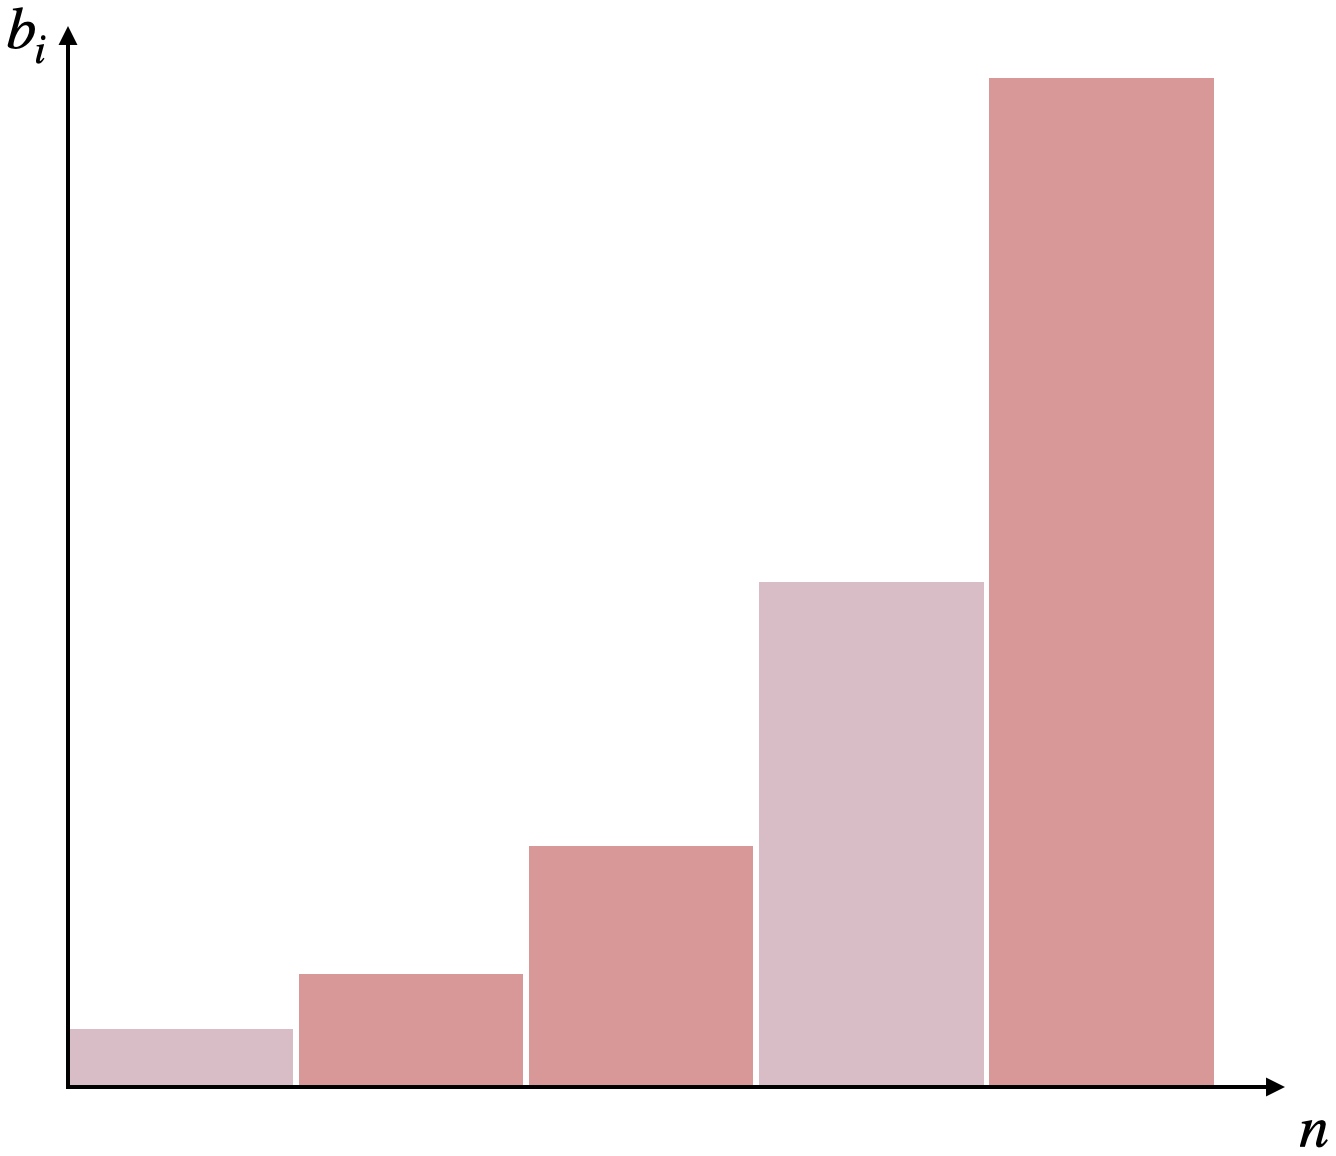
\includegraphics[width=\linewidth]{1PO}
\caption{PO}\label{AAA}
\end{subfigure}\hfill
\begin{subfigure}[b]{.49\linewidth}
\centering
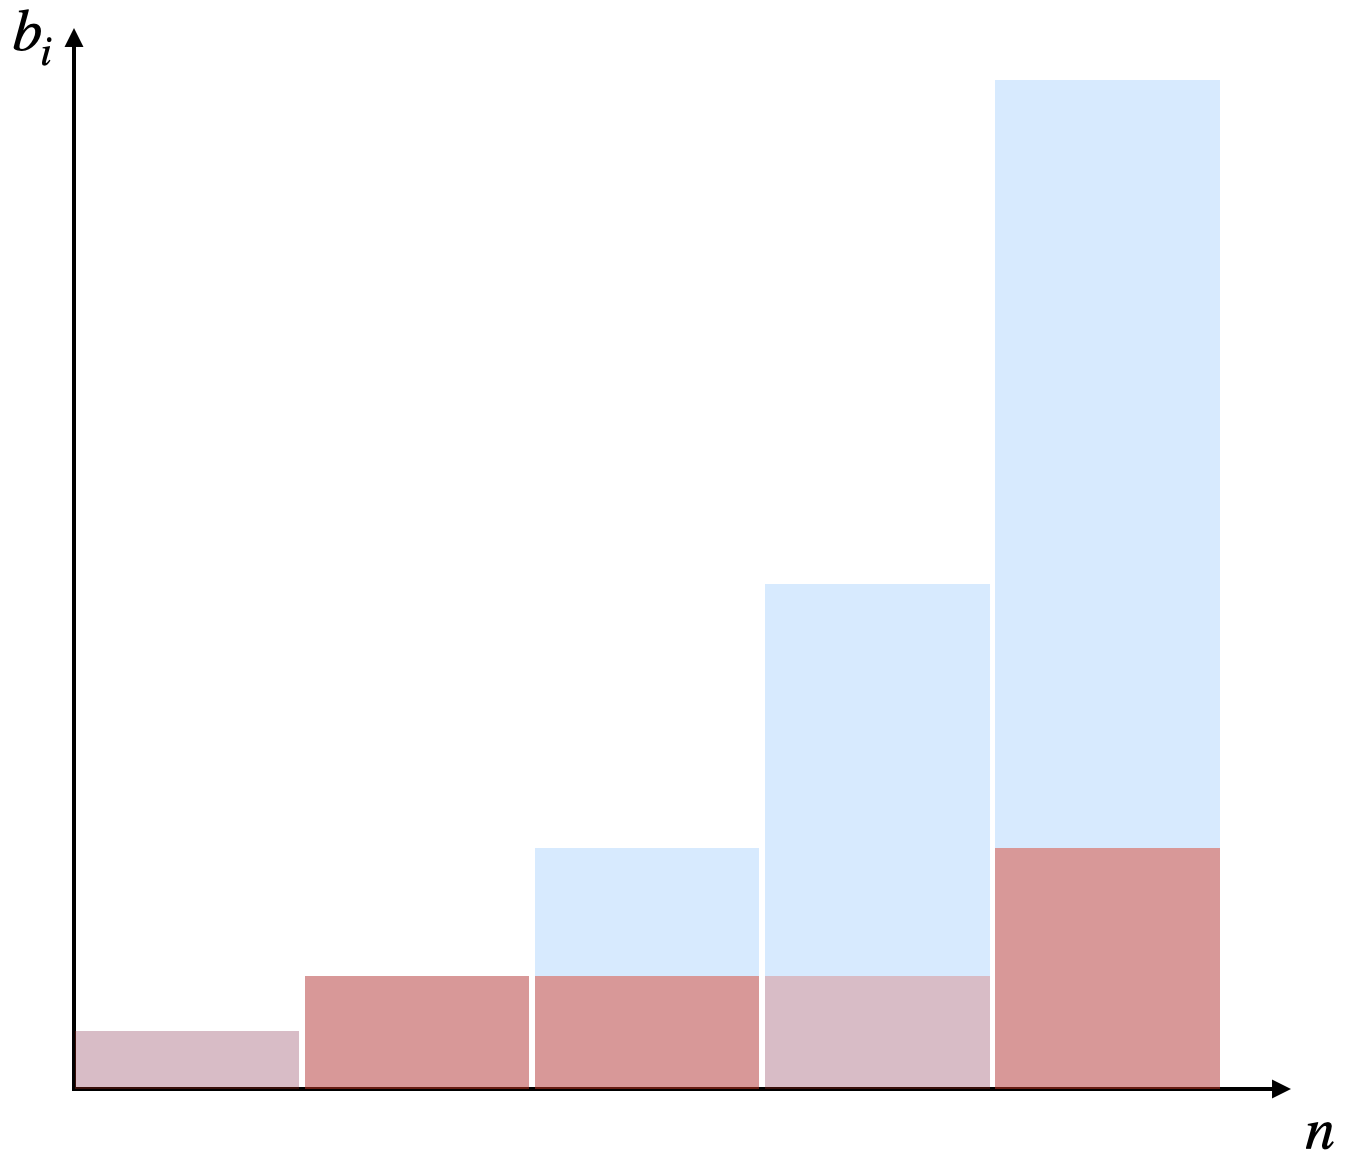
\includegraphics[width=\linewidth]{1PtQ}
\caption{PtQ}\label{BBB}
\end{subfigure}%
%\caption{name A and B \subref{AAA}\subref{BBB}}
\end{figure}
\vspace{-0.5em}
In PO,  5 experts undertake and receive bonuses sized with a full hierarchy of length 5.\\
In PtQ, 3 undertake, and the hierarchy reduces to 3 =  (5 - 3 + 1).
\end{frame}



\begin{frame}{PO vs.\ PtQ: When 5/5 need fixing}

\begin{figure}[h!]
\begin{subfigure}[b]{.49\linewidth}
\centering
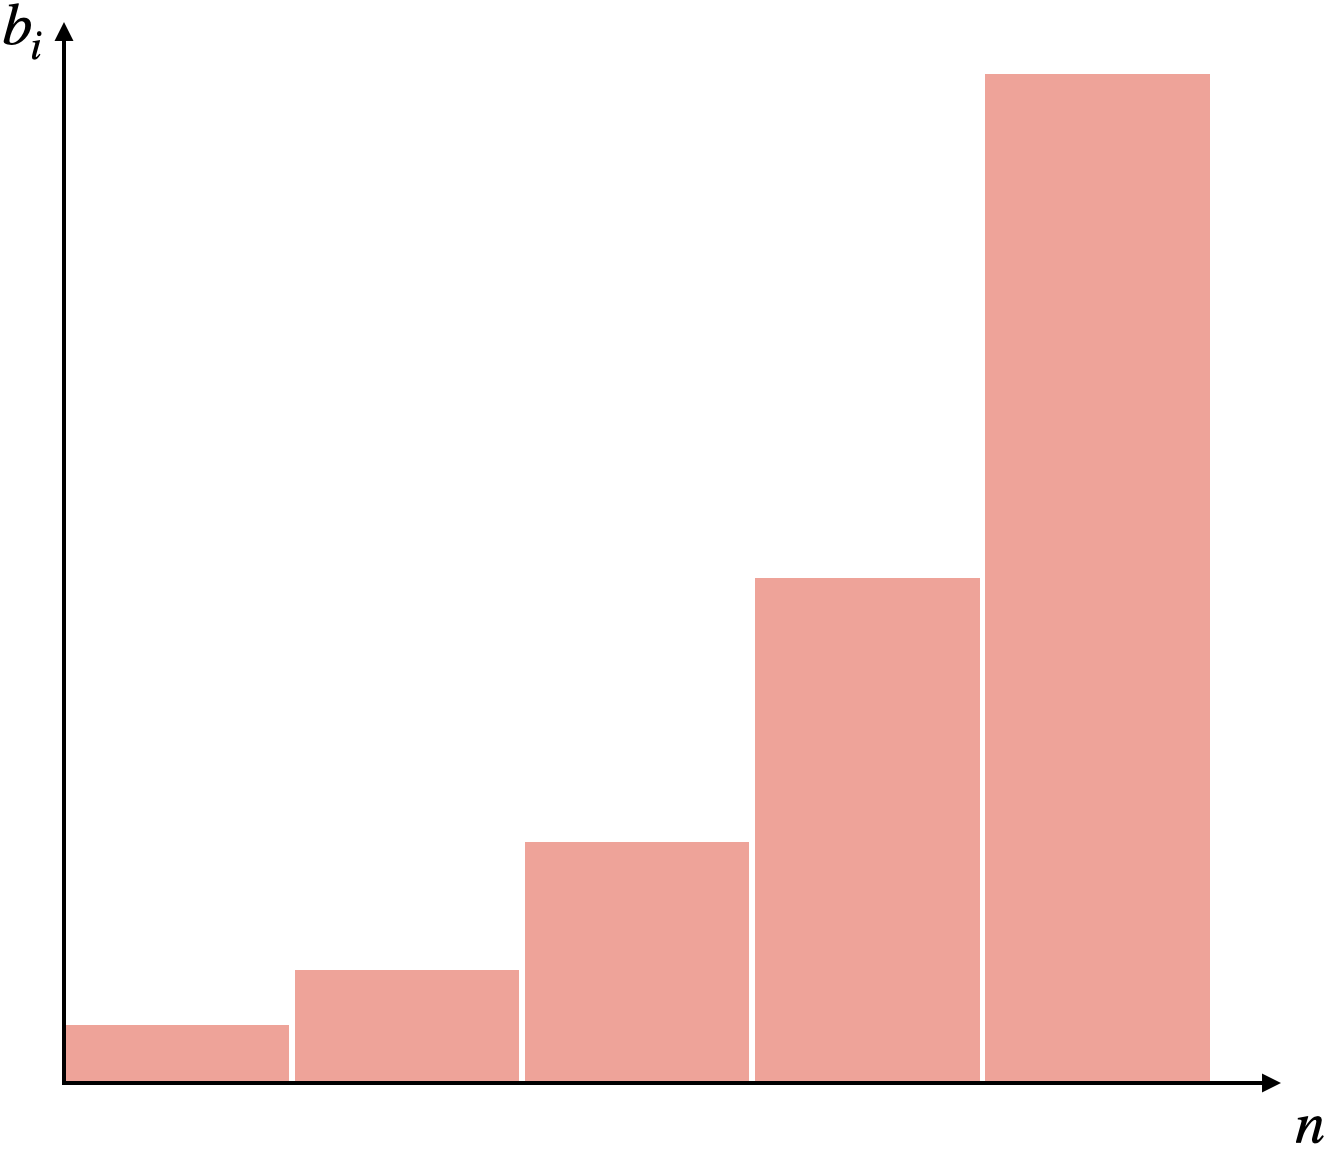
\includegraphics[width=\linewidth]{2PO}
\caption{PO}\label{AAA}
\end{subfigure}\hfill
\begin{subfigure}[b]{.49\linewidth}
\centering
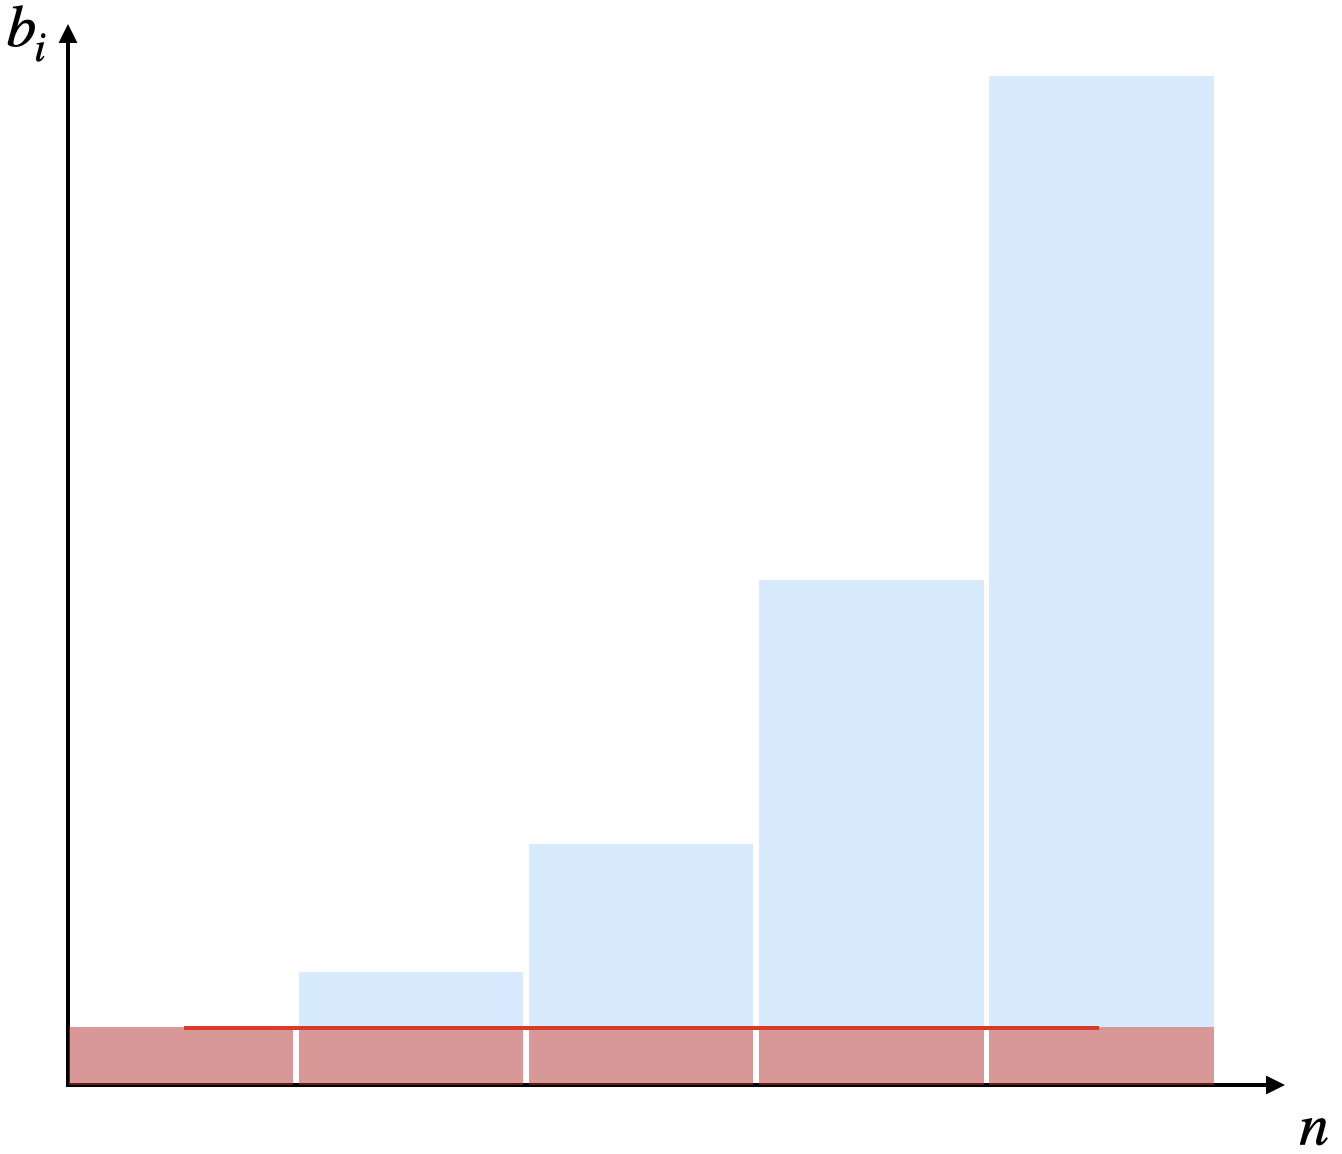
\includegraphics[width=\linewidth]{2PtQ}
\caption{PtQ}\label{BBB}
\end{subfigure}%
%\caption{name A and B \subref{AAA}\subref{BBB}}
\end{figure}
\vspace{-0.5em}
In PO,  5 experts undertake and receive bonuses sized with a full hierarchy of length 5.\\
In PtQ, 5 undertake, and the hierarchy reduces to 1 = (5 - 5 + 1).



\end{frame}





\begin{frame}{PO vs.\ PtQ: When 0/5 need fixing}
\begin{figure}[h!]
\begin{subfigure}[b]{.49\linewidth}
\centering
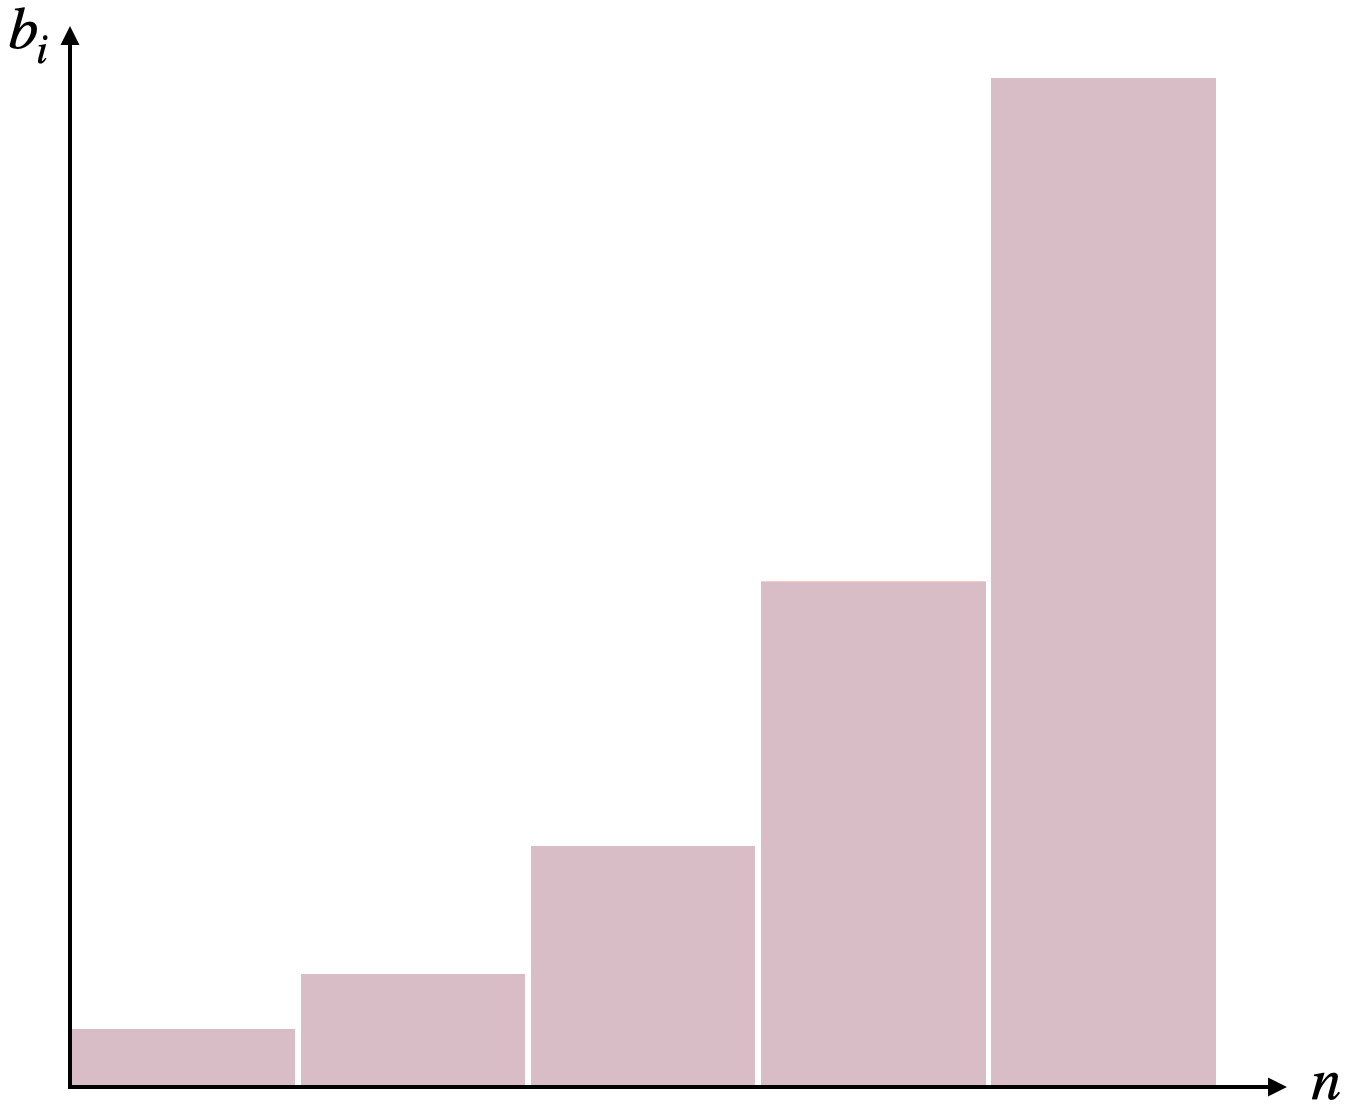
\includegraphics[width=\linewidth]{3PO}
\caption{PO}\label{AAA}
\end{subfigure}\hfill
\begin{subfigure}[b]{.49\linewidth}
\centering
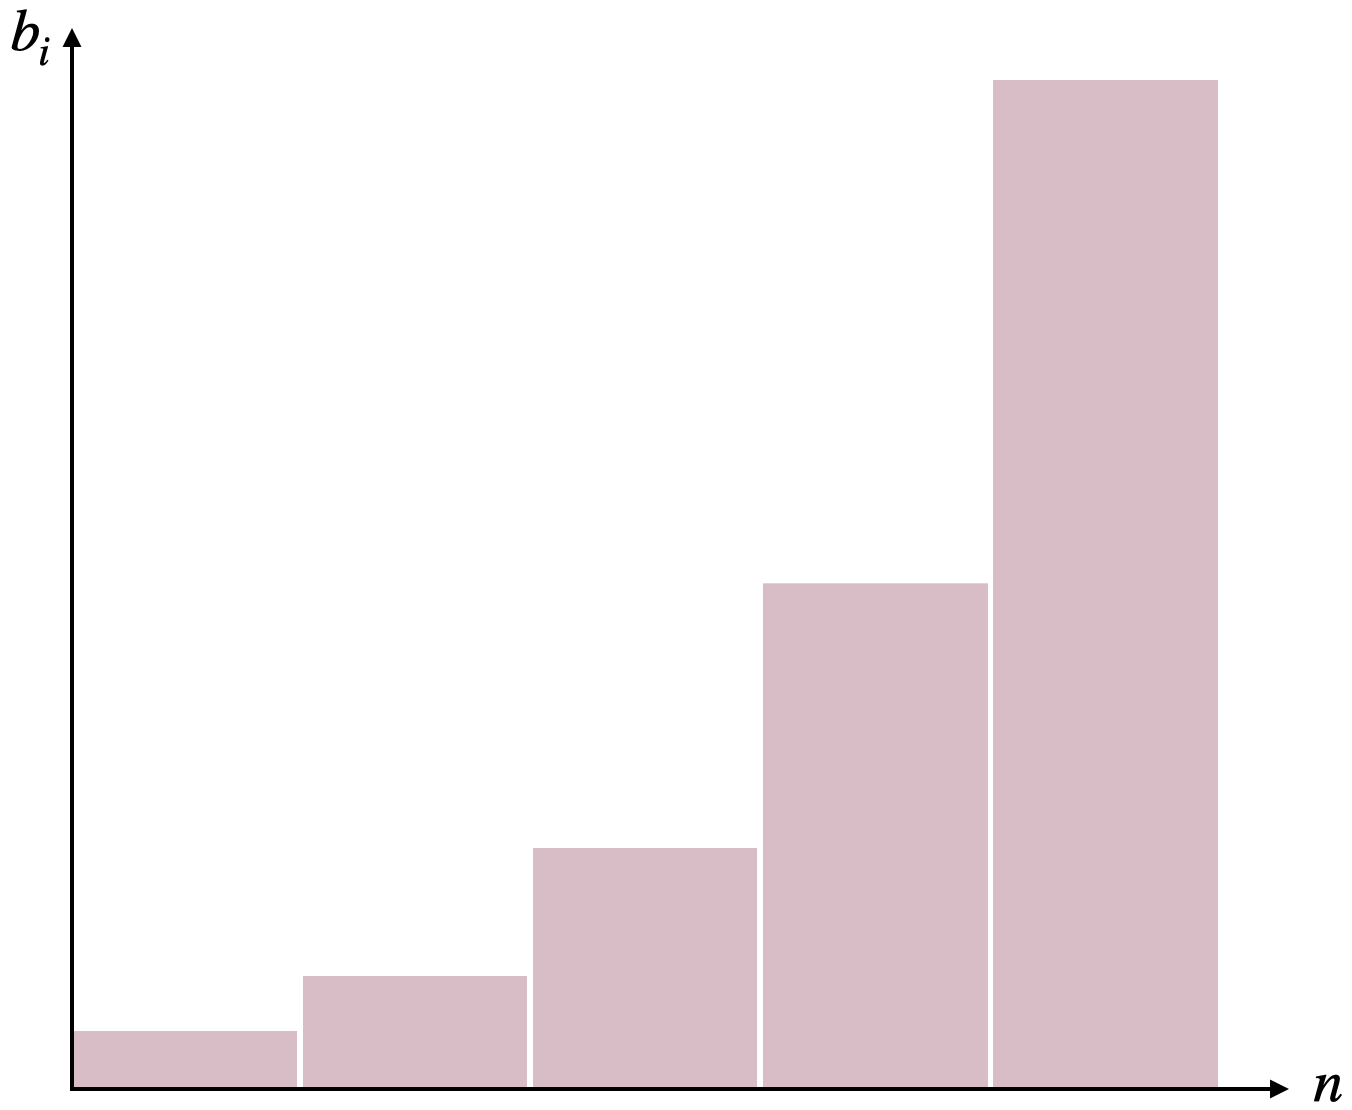
\includegraphics[width=\linewidth]{3PtQ}
\caption{PtQ}\label{BBB}
\end{subfigure}%
%\caption{name A and B \subref{AAA}\subref{BBB}}
\end{figure}
\vspace{-0.5em}
In PO,  5 experts undertake and receive bonuses sized with a full hierarchy of length 5.\\
In PtQ, 5 opt out, and the hierarchy is of full length 5.


\end{frame}






\begin{frame}{Why is PtQ optimal?}

{Contracts} robustly implementing all-high-quality
\smallskip

\begin{itemize}
  \item
 need {not} be uniformly PO or PtQ across experts and undertaking profiles, $(i,\mathbf a_{-i})$,\\[0.5em]
\item
but at each $(i,\mathbf a_{-i})$, $\mathbf b$ must either \emph{pool} or \emph{separate} $i$'s type.\\[0.5em]

\end{itemize}
\smallskip

The design is a {local} choice between PO and PtQ.

\bigskip

\smallskip

\textbf{Key spillover:}\quad At each $(i, \mathbf a_{-i})$, switching from PO to PtQ
\smallskip

\begin{itemize}
  \item is \emph{free} for the principal,
  \item makes undertaking \emph{informative} about high quality,
  \item \emph{lowers} the bonuses required by experts resolved earlier than $i$ in the elimination order.
\end{itemize}

\end{frame}





\begin{frame}[label=optcontract]{Optimal contract}

The logic extends to $n$ experts with heterogeneous $c_i$ and str. inc. and str. supermodular $P(Q)$.

\medskip

The problem collapses to finding an {optimal order} of eliminations:
$$\displaystyle\sigma^* \in \argmin_{\sigma\in\mathrm{Perm}(N)} C^{\mathrm{PtQ}}(\sigma,\mathbf p)$$

\bigskip

\begin{proposition}[Optimal UI contract]
The optimal contract among contracts that robustly implement all-high-quality is a PtQ contract for all $(i, \mathbf a_{-i})$, for some $\sigma \in \mathrm{Perm}(N)$.
\end{proposition}

\medskip

In general, $\sigma^*$ admits no closed-form characterization.
\hfill\hyperlink{proofsketch}{\beamergotobutton{Proof sketch}}
\smallskip

In O-ring production, the optimal order ranks experts who are cheap / critical / likely-already-satisfactory earlier.
\end{frame}








\begin{frame}{Final remarks}


Result.
\smallskip

The optimal contract pays experts to opt out while robustly inducing repair of every faulty part.

    \bigskip

Mechanism.
\smallskip

The incentive scheme makes an already observable choice informative.

    \bigskip


Team spillover.
\smallskip

Making one expert's choice informative lowers the bonuses needed to incentivize other experts. The value of separation extends beyond the expert being separated.


\end{frame}






\begin{frame}{Related literature}
\small

{Contracting with externalities}
\begin{itemize}
  \item Segal (2003): divide-and-conquer under multilateral externalities
  \item Bernstein \& Winter (2012): heterogeneous participation externalities
\end{itemize}

\medskip

{Team moral hazard with complementarities}
\hfill {\footnotesize unique implementation under action uncertainty}
\begin{itemize}
  \item Winter (2004): hierarchical contracts
  \item Halac, Lipnowski \& Rappoport (2021): principal-designed uncertainty
\end{itemize}

\medskip

{Robust implementation}
\hfill {\footnotesize robust to beliefs about types}
\begin{itemize}
  \item Bergemann \& Morris (2017); Dekel, Fudenberg \& Morris (2007)
\end{itemize}

\medskip

{Mechanism design with evidence}
\hfill {\footnotesize exogenous evidence structure}
\begin{itemize}
 \item Green \& Laffont (1986); Bull \& Watson (2007)
\end{itemize}

\bigskip

{This paper:} unique implementation robust to \emph{both} type and action uncertainty, \\
\quad\quad\quad\quad\quad with \emph{endogenous} evidence created through contract design.

\end{frame}





%=============================================================
% BACKUP
%=============================================================

\appendix
\backupbegin


\begin{frame}[plain, noframenumbering]
\centering
\vfill
{\large Appendix}
\vfill
\end{frame}



%=============================================================
% APPENDIX (secondary results)
%=============================================================





\begin{frame}[noframenumbering, label=BFRdef]{Belief-Free Rationalizability}

{\small
\begin{definition}[Belief-free rationalizable actions]
\textbf{Initialize:} $B^{\mathbf{b}}_{i,0}(\theta_i) = \mathcal{A}_i = \{(0, S),\, (1, S),\, (1, W)\}$ for all $i \in N$, $\theta_i \in \Theta$.
\vspace{0.2em}

\textbf{Iterate:} $(a_i, e_i) \in B^{\mathbf{b}}_{i,k}(\theta_i)$ survives in $B^{\mathbf{b}}_{i,k+1}(\theta_i)$ iff there exists an arbitrary conjecture $\nu \in \Delta(\Theta_{-i} \times \mathcal{A}_{-i})$ such that:
\begin{enumerate}
  \item[(i)] $\nu(\boldsymbol{\theta}_{-i}, \mathbf{a}_{-i}, \mathbf{e}_{-i}) > 0 \Rightarrow (a_j, e_j) \in B^{\mathbf{b}}_{j,k}(\theta_j)$ for all $j \neq i$;
  \item[(ii)] $(a_i, e_i) \in \arg\max_{(a_i', e_i') \in \mathcal{A}_i} \sum u_i^{\mathbf{b}}(\theta_i, a_i', e_i' \mid \boldsymbol{\theta}_{-i}, \mathbf{a}_{-i}, \mathbf{e}_{-i})\, \nu(\cdot)$.
\end{enumerate}
\vspace{0.2em}
\textbf{Limit:} $B_i(\theta_i \mid \mathbf{b}) = \bigcap_{k \geq 0} B^{\mathbf{b}}_{i,k}(\theta_i)$.
\end{definition}
}

\hfill\hyperlink{solutionconcept}{\beamerreturnbutton{Back}}
\end{frame}






\begin{frame}[label=proofsketch]{Optimal contract: Proof sketch}

Idea: 
Start from any contract.\\
We can always find a PtQ contract that is cheaper for each realization.
\bigskip

{\footnotesize Start from any robust all-high-quality contract $\mathbf b$:

\begin{enumerate}
  \item \textcolor{blue}{Characterize}: Let  $\tau(i)$=the elimination round for Expert $i$ and $S_i(\mathbf a_{-i})$=the assured sets.
  \smallskip
  \item \textcolor{blue}{Fill in}: Choose a ranking $\sigma$ refining (breaking ties in) $\tau$. \\
  				Extend bonuses to all off-path profiles (unreachable) at critical values \hfill $\Rightarrow$ same cost.
  \smallskip
  \item \textcolor{blue}{Reduce}: Replace bonuses with critical values along $\sigma$ \hfill $\Rightarrow$ weakly lower cost.
  \smallskip
  \item \textcolor{blue}{Switch to PtQ}: expert by expert, PO-form $\to$ PtQ-form \\
  Each switch preserves UI and enlarges predecessors' assured sets
   \hfill $\Rightarrow$ weakly lower cost.
  \smallskip
  \item \textcolor{blue}{Optimize}: $\ C(\mathbf b) \geq C^{PtQ}(\sigma,\mathbf p) \geq \min_{\sigma'} C^{PtQ}(\sigma',\mathbf p)$.
\end{enumerate}
}



\hfill\hyperlink{optcontract}{\beamerreturnbutton{Back}}
\end{frame}




\begin{frame}{General setting}

\textbf{Environment}
\begin{itemize}
  \item $n$ experts, heterogeneous type dist. $p_i = \Pr(\theta_i = H) \in (0,1)$ and effort costs $c_i > 0$
  \item Success probability $P(Q)$ is \emph{strictly increasing} and \emph{strictly supermodular} in the high-quality set $Q$:
  \[
    P(Q\cup\{i\})-P(Q)\;<\;P(Q'\cup\{i\})-P(Q')
    \qquad \forall\, i,\ Q\subsetneq Q'\subseteq N\setminus\{i\}
  \]
\end{itemize}

\vspace{1.5em}

\textbf{Robust implementation (RI):}\quad $\mathbf b$ makes all-high-quality the \emph{unique} BFR outcome.\\[0.3em]
\textcolor{gray}{\small (up to a vanishing tie-breaking perturbation, since the RI set is typically open)}

\vspace{1.5em}

\textbf{Optimal RI contract}
$$\min_{\mathbf b\,\in\,\mathrm{RI}}\ P(N)\,\mathbf E_{\mathbf p}\!\left[\sum_{i\in N} b_i\big(\mathbf a(\mathbf\theta)\big)\right]$$

\end{frame}




\begin{frame}[noframenumbering]{PtQ: General characterization}

$$b_i^* = \frac{c_i}{P(W_{-i} \cup \{i\} \cup R_{<i}^{\sigma}) - P(W_{-i} \cup R_{<i}^{\sigma})}$$
where $W(\mathbf{a}) = \{j \in N: a_j = 1\}$ is the set of participants who are guaranteed to work{ and hence produce} $q_H$,
and \\
$R_{<i}^{\sigma}$ is the {set of} resolved experts before Expert $i$.
\vspace{0.8em}


\textbf{Perturbations:} Set $b_i(1, \mathbf{a}_{-i}) = b^*_i + \varepsilon_{i,1}$ and $b_i(0, \mathbf{a}_{-i}) = b^*_i + \varepsilon_{i,0}$.
\vspace{0.4em}

{\footnotesize
$$1 < \frac{\varepsilon_{i,0}}{\varepsilon_{i,1}} < \frac{P(W_{-i} \cup \{i\} \cup R^\sigma_{<i} ) }{P(W_{-i} \cup R^\sigma_{<i})} \qquad \forall\, \mathbf{a}_{-i}$$
}

must hold to break ties to induce the desired action for each type.

\vspace{0.8em}

By strict monotonicity, $\frac{P(W_{-i} \cup \{i\} \cup R^\sigma_{<i} ) }{P(W_{-i} \cup R^\sigma_{<i})} > 1$ for all $\mathbf{a}_{-i}$. Such perturbations always exist.

\end{frame}











\begin{frame}[noframenumbering, label=oring]{Special case: O-ring production}

\textbf{O-ring technology:}\quad $P(Q) = \prod_{i\notin Q}\lambda_i$, \ $0<\lambda_i < 1$\\[0.2em]
Every expert is a ``generalist'': $i$'s marginal contribution $\propto P(Q_{-i})$.

\medskip

\textbf{Closed form:}\quad Each later-resolved $j$ inflates every predecessor's bonus by a loading $\kappa_j := (1-p_j) + \dfrac{p_j}{\lambda_j} > 1$:
$$b_{\sigma(i)}^* = \underbrace{\frac{c_i}{1-\lambda_i}}_{\text{base bonus}}\ \prod_{\sigma(j)>\sigma(i)}\kappa_j$$

\begin{proposition}[Optimal ranking under O-ring]
The optimal contract ranks experts by \emph{increasing} priority index
$\displaystyle I_i = \frac{c_i\,\lambda_i}{p_i(1-\lambda_i)^2}$ and offers PtQ for each $(i, \mathbf a_{-i})$.
\end{proposition}

\medskip

{\small Rank early: \emph{cheap} (low $c_i$), \emph{critical} (low $\lambda_i$), \emph{likely-already-good} (high $p_i$).\\
Symmetric $\lambda$: $I_i \propto c_i/p_i$. \quad Symmetric $\lambda$ \& $c$: decreasing $p_i$ (most-likely-good first).}
\hfill\hyperlink{proofsketchORING}{\beamergotobutton{Proof}}
\end{frame}



\begin{frame}[noframenumbering]
{Fragile technology}

Intervention without care \emph{degrades} quality:
$$
q(\theta_i, a_i, e_i) = \begin{cases}
q_H & \text{if } \theta_i = H, a_i = 0 \\
q_H & \text{if } a_i = 1 \text{ and } e_i = W \\
q_L & \text{otherwise}
\end{cases}
$$

Now two contracts can separate types:

\medskip

\textbf{Contract 1 (PtQ):} $b_i(0, \mathbf{a}_{-i}) > b_i(1, \mathbf{a}_{-i})$ \quad (same as before)
\begin{itemize}
  \item Participants = assured high quality.  Better when defects are common.
\end{itemize}

\medskip

\textbf{Contract 2 (PtP):} $b_i(1, \mathbf{a}_{-i}) > b_i(0, \mathbf{a}_{-i}) > b_i(1, \mathbf{a}_{-i}) - c_i$
\begin{itemize}
  \item Non-participants = assured high quality. Better when parts are mostly stable.
  \item 	After type separation, hierarchical wage sizing for participants
\end{itemize}

\medskip

Optimal: assign PtQ when $p_i \leq 1/2$, PtP when $p_i > 1/2$.

\end{frame}










\begin{frame}[noframenumbering, label=proofsketchORING]{O-Ring characterization proof}

Under $P(Q) = \prod_{i \notin Q} \lambda_i$, expected cost under ranking $\sigma$:
$$C^{PtQ}_{\mathbf{p}}(\sigma)
= \sum_{k=1}^{n} \frac{c_{i_k}}{1 - \lambda_{i_k}} \prod_{\ell > k} \kappa_{i_\ell},
\qquad \kappa_i := (1 - p_i) + \frac{p_i}{\lambda_i}$$

\medskip

Adjacent swap condition: rank $i$ before $j$ iff
$\displaystyle\frac{c_i/(1-\lambda_i)}{\kappa_i - 1} \leq \frac{c_j/(1-\lambda_j)}{\kappa_j - 1}$.

\medskip

$\Longrightarrow$ Optimal ranking: increasing $I_i = \dfrac{c_i \, \lambda_i}{p_i(1-\lambda_i)^2}$.

\hfill\hyperlink{oring}{\beamerreturnbutton{Back}}
\end{frame}




\backupend

\end{document}



\iffalse
Second, for the special case when the low-congruence employee is very unproductive on the
high-impact project, another common implementation of a fixed salary is the use of severance
pay. Contracts that include severance, golden parachutes, or “pay-to-quit” provisions specify a
payment made to the employee if he or she leaves the organization. In this case, the low-impact
project can be interpreted as the firm’s value from being able to replace the current employee.
For instance, organizations usually have only one department chief for each department. Yet, in
the case of an acquisition, the acquiring firm may have gained several qualified candidates to
potentially head one of its departments. In that case, monetary compensation for quitting can be
used as a tool for a non-congruent department chief to self-select out of the organization. This
selection out of the firm is valuable, as the firm can then search for and appoint a congruent
employee for that opened position. Our results therefore suggest that severance or “pay-to-quit”
incentives are beneficial even when taken up before an employee starts to work on a project.
This complements existing insights in the literature, which have focused on using these contract
features to influence the employee’s choices during or after his or her work on projects (Dur and
Schmittdiel, 2019; Almazan and Suarez, 2003; Manso, 2011; Inderst and Mueller, 2010).

The management of talent: Optimal
contracting for selection and incentives
Dana Foarta∗
and
Takuo Sugaya∗
lit review에서 배껴옴.
severance, golden parachutes, or “pay-to-quit” 이런 단어를 쓰나봐 골든 패러슈트?



%여기에 amazon, 하고 딴 회사 이야기를 뉴스로 넣는건 어때?
https://hbr.org/2023/05/how-a-pay-to-quit-strategy-can-reveal-your-most-motivated-employees

``How a Pay-to-Quit Strategy Can Reveal Your Most Motivated Employees,'' \textit{Harvard Business Review}, May 2023.

\href{https://hbr.org/2023/05/how-a-pay-to-quit-strategy-can-reveal-your-most-motivated-employees}{Harvard Business Review, May 2023}

\citet{hbr2023payquit}




\fi






\iffalse
@misc{hbr2023payquit,
  author  = {Sucher, Sandra J. and Gupta, Shalene},
  title   = {How a Pay-to-Quit Strategy Can Reveal Your Most Motivated Employees},
  year    = {2023},
  howpublished = {Harvard Business Review},
  note    = {\url{https://hbr.org/2023/05/how-a-pay-to-quit-strategy-can-reveal-your-most-motivated-employees}},
}

@article{Dur2019PaidTQ,
  title={Paid to Quit},
  author={Robert Dur and Heiner Schmittdiel},
  journal={De Economist},
  year={2019},
  volume={167},
  pages={387 - 406},
  url={https://api.semanticscholar.org/CorpusID:154351458}
}

@article{Foarta2021TheMO,
  title={The management of talent: Optimal contracting for selection and incentives},
  author={Dana Foarta and Takuo Sugaya},
  journal={The RAND Journal of Economics},
  year={2021},
  url={https://api.semanticscholar.org/CorpusID:197871225}
}

@inproceedings{Castro2025IncSel,
  title={Incentives and Selection },
  author={Henrique Castro-Pires and George Georgiadis},
  url={https://api.semanticscholar.org/CorpusID:272856238}
}

\fi
